% !TEX root = mythesis.tex



%==============================================================================
\chapter{Analysis strategy}
\label{sec:analysisstrategy}
%==============================================================================
The purpose of this chapter is to provide a brief overview of the $T/Y\rightarrow Wb$ process. The contribution from the Standard Model backgrounds is discussed in detail in section \ref{sec:analysisstrategy:backgrounds}. The generators used for the production of MC samples are also outlined. Moreover, the physics objects are described in addition to the event selection used for this analysis. Finally, a motivation for the need of a data-driven method is given.

%------------------------------------------------------------------------------
\section{Overview of $T/Y\rightarrow Wb$ }%
\label{sec:analysisstrategy:t/y}
%------------------------------------------------------------------------------
The analysis concentrates on a search for single production of vector-like quarks $Q$ by the fusion of $W$ boson and $b$-quark in $pp$ collisions ($pp\rightarrow Qqb$) with a subsequent decay of $Q \rightarrow Wb$. Here $Q$ can either be $T$ quark, $Y$ quark or their antiquarks ($\bar{Q}=\bar{T}\text{ or }\bar{Y}$). Since it is an inclusive analysis so the search includes both the final states $W^{\text{+}}b$ and $W^{\text{-}}\bar{b}$ coming from the decay of $Q$ and $\bar{Q}$ respectively.

There are two decay modes of $W$ boson. It can either decay leptonically or hadronically depending on the branching fraction of a decay mode. The analysis targets two channels depending on the decay of $W$ boson. Both the channels are described in detail in the section below:


%------------------------------------------------------------------------------
\subsection{Leptonic channel}%
\label{sec:analysisstrategy:leptonicchannel}
%------------------------------------------------------------------------------
This section describes the leptonic channel of $T/Y\rightarrow Wb$ process. In this, $W$ boson decays leptonically, giving a lepton + jets signature which is characterised by the presence of exactly one electron (or muon), two (or more jets) and missing transverse momentum from the neutrino.~\cite{vlqpaper}. A leading-order (LO) Feynman diagram for the leptonic channel is shown in Fig.\ \ref{fig:analysisstrategy:leptonicchannel}. 

\begin{figure}[hbt!]
	\centering
	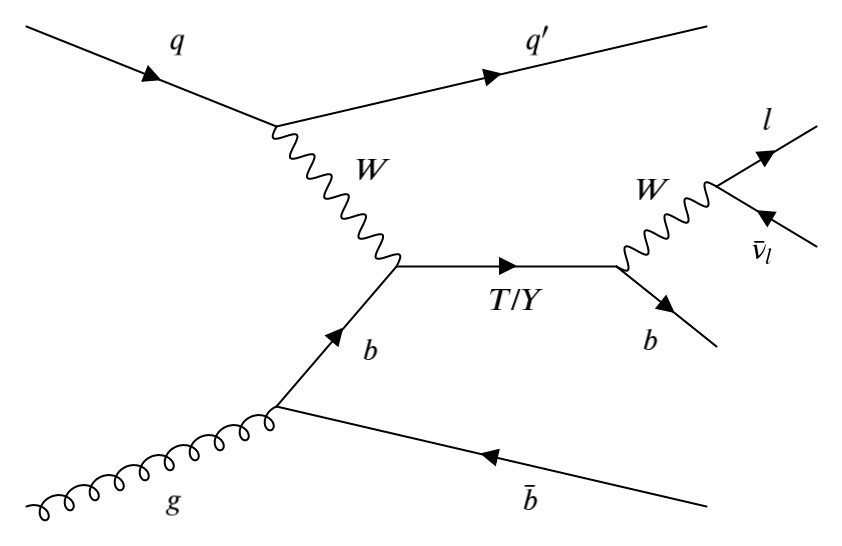
\includegraphics[width=0.6\linewidth]{twbleptonic.png}
	\caption{A leading-order Feynman diagram for single production of $T/Y$ quark in $pp \rightarrow Q\rightarrow Wb$ process where $W$ boson further decays leptonically.}
	\label{fig:analysisstrategy:leptonicchannel}
\end{figure}

The main background processes from a single-lepton signature arise from ($t\bar{t}$), single top and $W$ boson production in association with jets ($W$+jets), with smaller contributions from $Z$ boson production in association with jets ($Z$+jets) and diboson ($WW$, $WZ$, $ZZ$) production. Multijet events can also contribute to the background if a jet is misidentified as an electron or non-prompt electron (or muon).~\cite{vlqpaper} Processes like $t\bar{t}W$, $t\bar{t}Z$ and $t\bar{t}H$ are also considered which can also produce a very small effect to the background.

The analysis for leptonic channel with the ATLAS 2015-16 data corresponding to integrated luminosity of $\SI{36.1}{\femto\barn^{\text{-1}}}$ results in setting the mass-coupling limits.~\cite{vlqpaper} Fig.\ \ref{fig:analysisstrategy:leptonicchannel:limit} shows 95\% confidence level (CL) limits on cross-section times branching ratio of the right-handed $Y$ quark for a ($B,Y$) doublet model as a function of VLQ mass. The branching ratio $\mathcal{B}(Y\rightarrow Wb)$ is set to one for theoretical predictions. The area above the solid line gives the excluded region. This result is from the previous analysis and now a new analysis with the ATLAS 2015-18 data corresponding to an integrated luminosity of $\SI{139.1}{\femto\barn^{\text{-1}}}$ with better and improved methods is also being done.


\begin{figure}[hbt!]
	\centering
	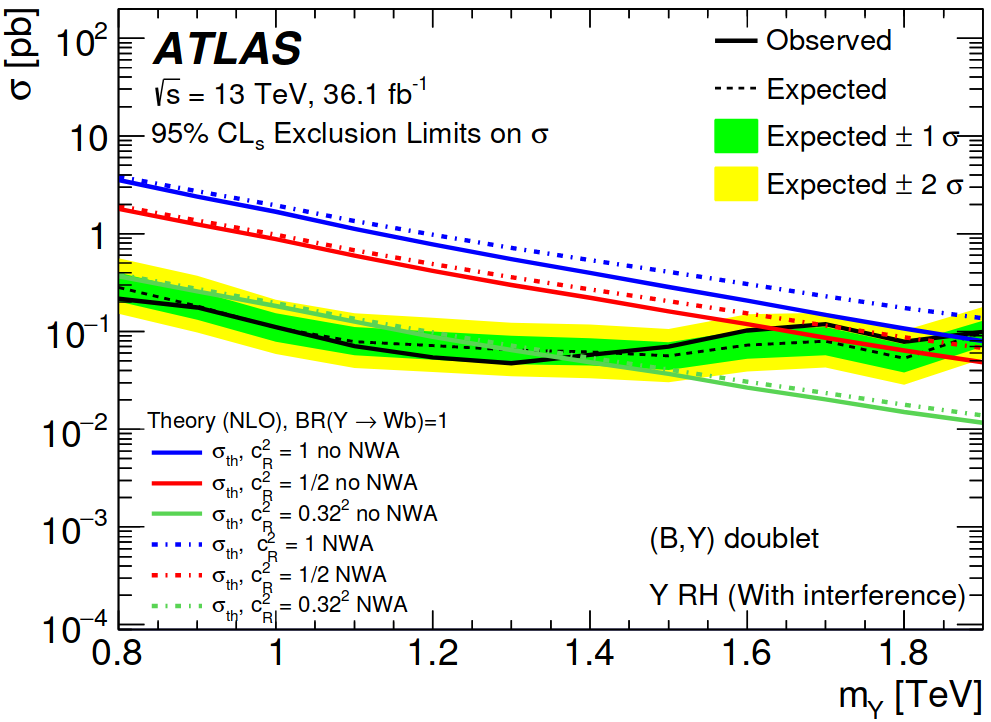
\includegraphics[width=0.55\linewidth]{masslimit.png}
	\caption{The expected and observed 95\% CL limits for right-handed $Y$ quark from ($B,Y$) doublet as a function of VLQ mass are shown for cross-section times branching ratio $\mathcal{B}(Y\rightarrow Wb)$.~\cite{vlqpaper}}
	\label{fig:analysisstrategy:leptonicchannel:limit}
\end{figure}

%------------------------------------------------------------------------------
\subsection{Hadronic channel}%
\label{sec:analysisstrategy:hadronicchannel}
%------------------------------------------------------------------------------
This channel is optimised to a search for $T/Y$ quark which decays into a high $p_{\text{T}}$ $W$ boson and $b$-quark, where $W$ boson decays hadronically. Both $W$ boson and $b$-quark are approximately back-to-back in the transverse plane since both originate from the decay of heavy particle. Fig.\ \ref{fig:analysisstrategy:hadronicchannel} shows a leading-order Feynman diagram of the hadronic decay of $W$ boson in $T/Y \rightarrow Wb$ process. There is an additional $b$-quark which is produced from the gluon splitting can be observed in either the forward or central region. This $b$-quark usually produces a jet of low energy which falls outside the acceptance region of the detector. There is also a light-flavour quark $q'$ in the process which often produces a jet in the forward region of the detector.

\begin{figure}[hbt!]
	\centering
	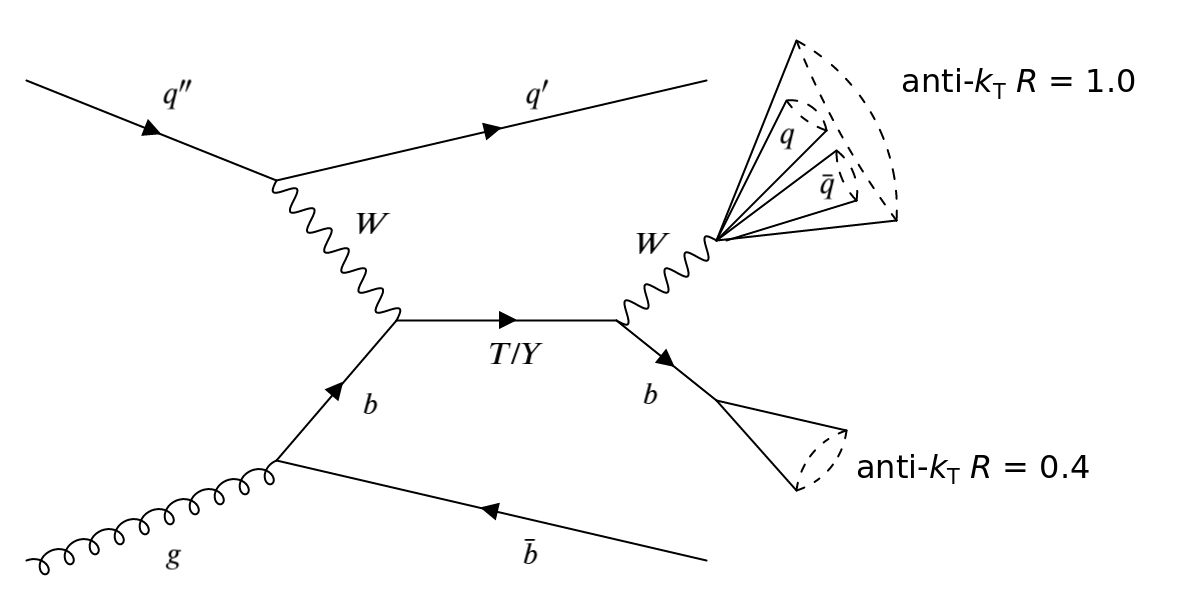
\includegraphics[width=0.8\linewidth]{twbhadronic.png}
	\caption{A leading-order Feynman diagram for single production of $T/Y$ quark in $pp \rightarrow Q\rightarrow Wb$ process where $W$ boson further decays hadronically.}
	\label{fig:analysisstrategy:hadronicchannel}
\end{figure}

All the main backgrounds with an all-jets signature arising from different SM processes are described in section \ref{sec:analysisstrategy:backgrounds}.


%------------------------------------------------------------------------------
\subsection{Motivation for hadronic channel}%
\label{sec:analysisstrategy:motivation}
%------------------------------------------------------------------------------
This thesis is focused on the hadronic channel of $T/Y\rightarrow Wb$. So, it is important to mention why it is interesting to study this decay mode. Some of the important points are described below:
\begin{itemize}
	\item $W$ boson is a vector boson, which has a very short lifetime. This means that within the ATLAS detector, it is never observed directly, only the decay products can be measured. $W$ boson decays into two fermions, i.e.\ either into a lepton and anti-neutrino ($\Plepton\APnulepton$) or a quark anti-quark ($q\bar{q}$) pair, where \Plepton includes all the three lepton flavours (\Pelectron, \Pmuon and \Ptauon). The branching fraction of $\mathcal{B}(W\rightarrow q\bar{q})$ is higher than $\mathcal{B}(W\rightarrow \Plepton\APnulepton)$, which makes the hadronic decay of $W$ boson an interesting channel to probe the kinematics of an analysis. 
	
	\item The decay of a heavy particle $T/Y$ produces high \pt $W$ boson and $b$-quark. So, the hadronic decay products of $W$ boson are boosted, which allow us to use large-$R$ jets to reconstruct $W$ boson. It also allows to use the taggers developed for such decays. Two of these taggers which are used in this analysis are already discussed in section \ref{sec:jetsandtaggers:taggers}. 
	
	\item Moreover, the leptonic analysis with 2015-18 ATLAS data for setting mass-coupling limits is being done. So, an addition of hadronic analysis is used to increase the sensitivity.~\cite{leptonic:twiki}
\end{itemize}


%------------------------------------------------------------------------------
\section{Backgrounds}%
\label{sec:analysisstrategy:backgrounds}
%------------------------------------------------------------------------------
This section covers all the possible backgrounds which are significant for the hadronic channel of $T/Y\rightarrow Wb$ that are studied for this analysis. The final state consists of $W$ boson with $b$-quarks, which resembles with the final state of many SM processes, for example, single top, $t\bar{t}$, $W$ boson and $Z$ boson accompanied with jets and multijet, which is a dominant background. The samples which are used to predict these backgrounds are produced from the Monte Carlo (MC) simulation, which is described in detail in section \ref{sec:analysisstrategy:mc:background}. The contribution from diboson processes ($WW$, $WZ$, $ZZ$) is negligible compared to the other backgrounds. Also, the MC samples for the hadronic decay of dibsoson process are not yet modelled. Therefore, they are not mentioned explicitly. 
%------------------------------------------------------------------------------
\subsubsection{Single top}%
\label{sec:analysisstrategy:singletop}
%------------------------------------------------------------------------------
Single top processes are the events in which top-quark is produced by the electroweak interaction. There are three main channels for the production of single top i.e.\ $s$-channel, $t$-channel and $tW$-channel. At the LHC, $t$-channel is a dominant process followed by $tW$-channel and then $s$-channel. In $tW$ production, the most distinct feature is a fermionic propagator. The $tW$ channel can be drawn as $s$-channel-like or $t$-channel-like. Fig.\ \ref{fig:analysisstrategy:singletop:s} shows a leading-order Feynman diagram of $s$-channel like $tW$ production, in which a bottom-quark first interacts with a gluon to become a virtual bottom-quark which then decays into $W$ boson and top-quark. Fig.\ \ref{fig:analysisstrategy:singletop:t} shows a leading-order Feynman diagram of $t$-channel like $tW$ production, in which a bottom-quark first emits a $W$ boson and turns to a virtual top-quark, which then interacts with a gluon to produce a top-quark. Both these diagrams require a bottom-quark inside a proton that means five flavours of parton should be treated as active inside a proton. It is known as a five-flavour scheme. The top-quark in both diagrams can further decay into $W$ boson and accompanied $b$-quark.~\cite{thesis:rui}  

\begin{figure}[hbt!]
	\centering
	\begin{subfigure}{.45\textwidth}
		\centering
		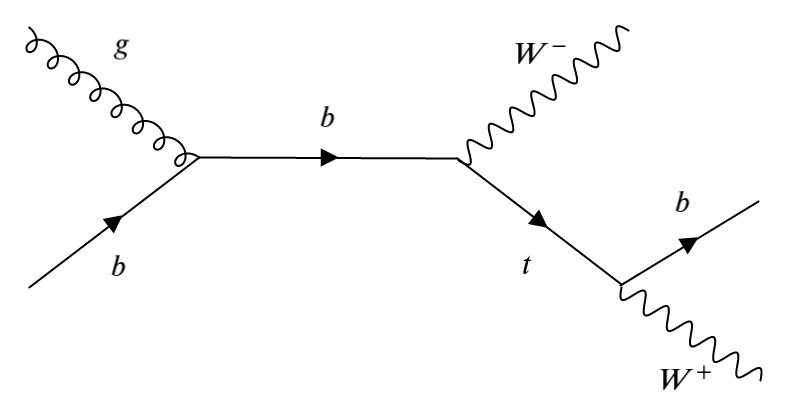
\includegraphics[width=\linewidth,height=\textheight,keepaspectratio]{singletop.png}\vspace{1.5cm}
		\caption{}
		\label{fig:analysisstrategy:singletop:s}
	\end{subfigure}\hspace{1cm}
	\begin{subfigure}{.3\textwidth}
		\centering
		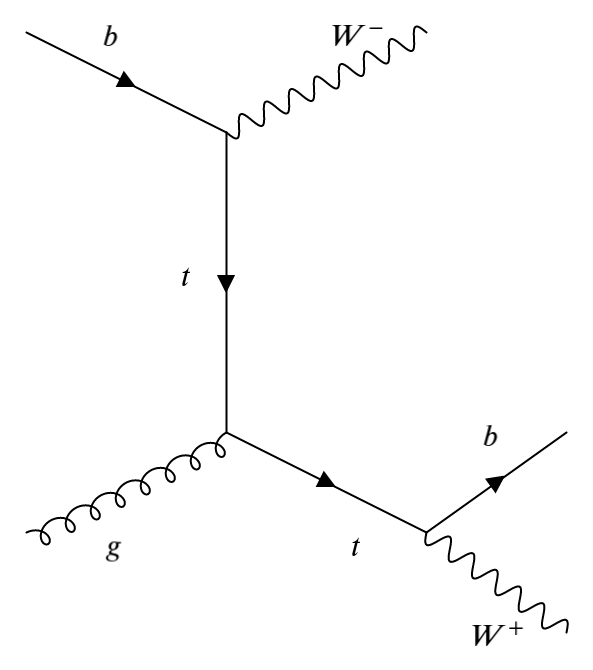
\includegraphics[width=\linewidth,height=\textheight,keepaspectratio]{singletop1.png}
		\caption{}
		\label{fig:analysisstrategy:singletop:t}
	\end{subfigure}
	\caption{A leading-order Feynman diagram of (a) $s$-channel like and (b) $t$-channel like $tW$ production in a five-flavour scheme.}
	\label{fig:analysisstrategy:singletop}
\end{figure}

%------------------------------------------------------------------------------
\subsubsection{\ensuremath{t\bar{t}}}%
\label{sec:analysisstrategy:ttbar}
%------------------------------------------------------------------------------
Top-quark pair production ($t\bar{t}$) can be produced either by gluon-gluon fusion ($gg$) or by annihilation of quark anti-quark pair ($q\bar{q}$). At the LHC, $gg$ fusion becomes a dominant process which contributes $\sim90\%$ of $t\bar{t}$ production. Some leading-order Feynman diagrams of $t\bar{t}$ production by $gg$ fusion are shown in Fig.\ \ref{fig:analysisstrategy:ttbar}. The final states $t$ and $\bar{t}$ can further decay into $\PWplus b$ and $\PWminus\bar{b}$ respectively and hence considered as one of the background processes for this analysis. The contribution from $t\bar{t}$ is higher than single top due to its larger production cross-section.~\cite{thesis:rui}


\begin{figure}[hbt!]
	\centering
	\begin{subfigure}{.45\textwidth}
		\centering
		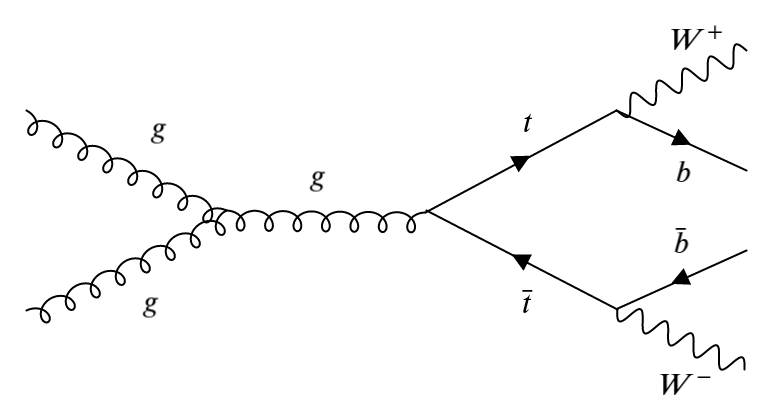
\includegraphics[width=\linewidth,height=\textheight,keepaspectratio]{ttbar.png}
		\caption{}
		\label{fig:analysisstrategy:ttbar1}
	\end{subfigure}\hspace{1cm}
	\begin{subfigure}{.4\textwidth}
		\centering
		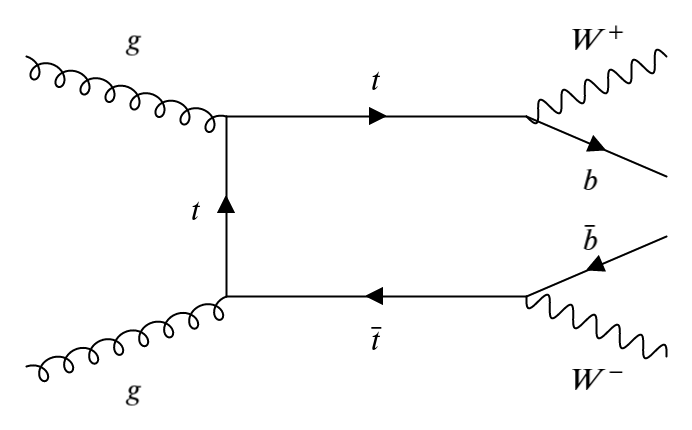
\includegraphics[width=\linewidth,height=\textheight,keepaspectratio]{ttbar1.png}
		\caption{}
		\label{fig:analysisstrategy:ttbar2}
	\end{subfigure}
	\caption{Some leading-order Feynman diagrams for $t\bar{t}$ production by $gg$ fusion.}
	\label{fig:analysisstrategy:ttbar}
\end{figure}

%------------------------------------------------------------------------------
\subsubsection{$W$+jets}%
\label{sec:analysisstrategy:w+jets}
%------------------------------------------------------------------------------
Another potentially significant background for the hadronic analysis is the production of $W$ boson accompanied by jets. An example of a corresponding Feynman diagram is shown in Fig. \ref{fig:analysisstrategy:wjets} where a quark first emits a $W$ boson, changes its flavour and turns into a virtual quark which further interacts with a gluon to give a quark which can be $b$-quark. So, this process also imitates the $T/Y\rightarrow Wb$ final state similar to single top production. $W$+jets process has significantly higher production-cross-section than single top and $t\bar{t}$.

\begin{figure}[hbt!]
	\centering
	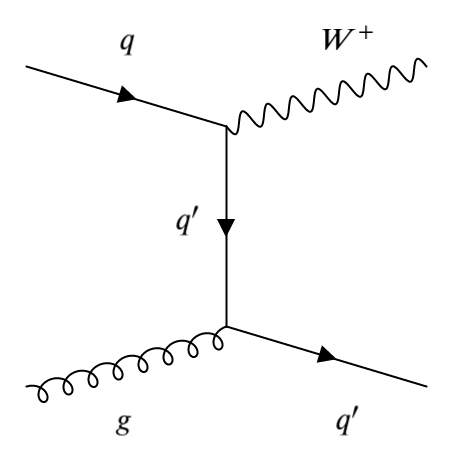
\includegraphics[width=0.35\linewidth]{wjets.png}
	\caption{A leading-order Feynman diagram for the production of $W$ boson accompanied by jets.}
	\label{fig:analysisstrategy:wjets}
\end{figure}

%------------------------------------------------------------------------------
\subsubsection{$Z$+jets}%
\label{sec:analysisstrategy:z+jets}
%------------------------------------------------------------------------------
This process includes the production of $Z$ boson accompanied by jets, where jets can be of any flavour. The branching ratio of $Z$ boson decaying into hadrons $\mathcal{B}(Z\rightarrow\text{ hadrons})$ $\sim70\%$. So, the contribution from $Z$+jets is significant for the background when $Z$ boson decays into $q\bar{q}$ with the accompanied jets to be $b$-jets. An example of a leading-order Feynman diagram for $Z$+jets process is shown in Fig.\ \ref{fig:analysisstrategy:zjets}. In this diagram, $Z$ boson is emitted from a quark which further annihilates with anti-quark to produce a gluon, which decays into $b\bar{b}$ pair.

\begin{figure}[hbt!]
	\centering
	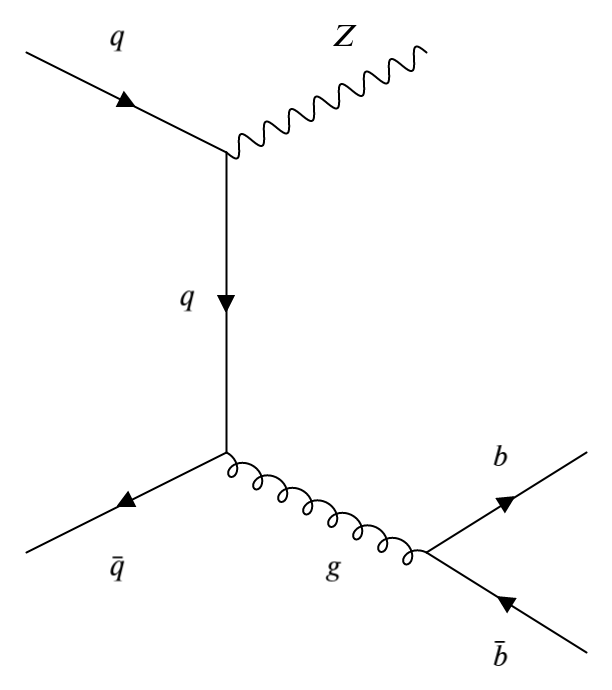
\includegraphics[width=0.33\linewidth]{zjets.png}
	\caption{A leading-order Feynman diagram for the production of $Z$ boson accompanied by jets.}
	\label{fig:analysisstrategy:zjets}
\end{figure}

%------------------------------------------------------------------------------
\subsubsection{Multijet}%
\label{sec:analysisstrategy:multijets}
%------------------------------------------------------------------------------
The hadronic channel is not a clean channel like leptonic channel because of the contribution from the QCD processes which accounts for a significant background. These QCD processes are very challenging because their theoretical prediction is so difficult to describe and also there are several experimental challenges associated with them. A detailed discussion on QCD has been outlined in section \ref{sec:theory:standardmodel:strong}.

In the $pp$ collision at $\sqrt{s}=\SI{13}{\tera\electronvolt}$, there is a lot of hadronic activity going on which constitute a large number of jets. Multijet include jets of any flavour. There are several ways for the production of multijet at the LHC. Some of them are depicted in Fig.\ \ref{fig:analysisstrategy:multijets}. These diagrams show the production of $q\bar{q}$ pair and $gg$ pair from gluon splitting. Multijet production has a higher cross-section in order of magnitude as compared to the other backgrounds. That is why multijet is the dominant background in the all-hadronic channel of this analysis. They have a problem with modelling because of the QCD processes.

\begin{figure}[hbt!]
	\centering
	\begin{subfigure}{.45\textwidth}
		\centering
		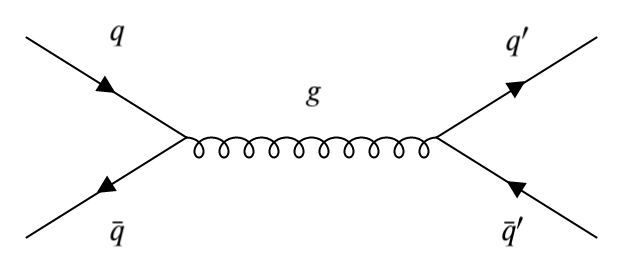
\includegraphics[width=\linewidth,height=\textheight,keepaspectratio]{multijets1.png}
		\caption{}
		\label{fig:analysisstrategy:multijets1}
	\end{subfigure}\hspace{0.5cm}
	\begin{subfigure}{.4\textwidth}
		\centering
		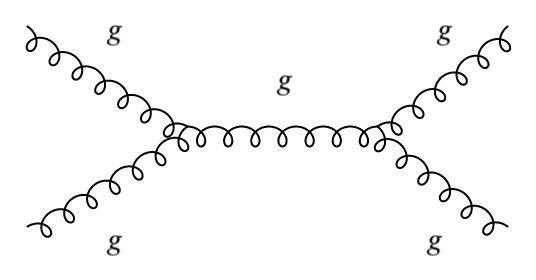
\includegraphics[width=\linewidth,height=\textheight,keepaspectratio]{multijets2.png}
		\caption{}
		\label{fig:analysisstrategy:multijets2}
	\end{subfigure}\hspace{0.5cm}
	\begin{subfigure}{.4\textwidth}
	\centering
	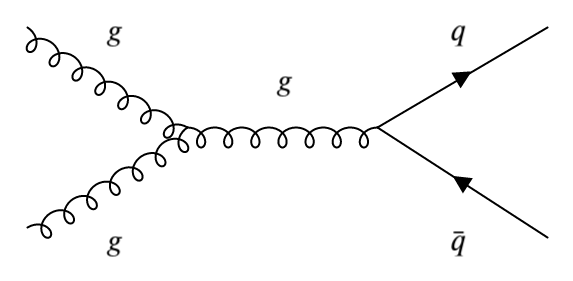
\includegraphics[width=\linewidth,height=\textheight,keepaspectratio]{multijets3.png}
	\caption{}
	\label{fig:analysisstrategy:multijets3}
	\end{subfigure}
\caption{Some examples of a leading-order Feynman diagram for multijet production from gluon splitting.}
\label{fig:analysisstrategy:multijets}
\end{figure}

%------------------------------------------------------------------------------
\section{Datasets}%
\label{sec:analysisstrategy:datasets}
%------------------------------------------------------------------------------

%------------------------------------------------------------------------------
\subsection{Data samples}%
\label{sec:analysisstrategy:datasets:data}
%------------------------------------------------------------------------------
In this thesis, full ATLAS Run 2 data have been used that means the data were collected from 2015 to 2018 with the ATLAS detector at $\sqrt{s}$ = 13 \si{\tera\electronvolt}. The selected data were recorded during stable LHC conditions and with the full functionality of the ATLAS detector. The data also fulfils the condition of \enquote{Good Run Lists (GRL)}. The GRL selects data where all of the detector systems were in good quality. Good quality means that all of the detectors were performing sufficiently well for the data to be used in physics analyses. The total amount of data satisfying these conditions correspond to a total integrated luminosity of $\SI{139}{\femto\barn^{\text{-1}}}$. The integrated luminosities of data obtained in different years are summed in Table \ref{table:analysisstrategy:datasets:data}.
\begin{table}[hbt!]
	\centering
	\begin{tabular}{c | c} 
		\toprule
		Data taken in & $\mathcal{L}_{\text{int}}$ (\si{\femto\barn^{\text{-1}}}) \\
		\midrule
		2015-16 & 36.2 \\
		2017 & 44.3 \\ 
		2018 & 58.5 \\ 
		\bottomrule
	\end{tabular}
	\caption{Integrated luminosities of the data for all the years of LHC Run 2 operation.~\cite{intnote:zboson}}
	\label{table:analysisstrategy:datasets:data}
\end{table}

%------------------------------------------------------------------------------
\subsection{Monte Carlo (MC) samples}%
\label{sec:analysisstrategy:mc}
%------------------------------------------------------------------------------
In order to study physics, a well-simulated sample is needed, which can predict the contribution from each background processes as well as the expected signal process. For this, the Monte-Carlo simulation is used, which is based on the stochastic methods to simulate various processes. They are used to predict event rates, simulate possible backgrounds, study detector effects, etc. The predictions from the MC samples can be then compared to the results achieved from the data.

The generation of MC samples is divided into three steps. First, the underlying events are generated using the help of a general-purpose event generator, e.g.\ \textsc{Sherpa}~\cite{sherpa}. After this, the hadronisation process of these events is simulated by the help of parton showering software. At last, these events are passed to the detector simulation software called \textsc{Geant4}~\cite{geant}, to simulate the detector effects as if it is passed to the real ATLAS detector to detect the particles. The last step includes either a full simulation or through a faster simulation making use of parameterised showers in the calorimeters. 

The effects of both in-time and out-of-time pile-up\footnote{In-time pile-up means additional $pp$ collisions in the same bunch crossings, and out-of-time pile-up means additional $pp$ collisions in the nearby bunch crossings.} have been modelled in the MC samples by reweighting. The reweighting is done to match the pile-up conditions observed in data taken in the respective year. The MC samples are modelled by following the common Physics Modelling Group (PMG) recommendations. 

MC samples simulating Run 2 conditions are divided into three campaigns, labelled MC16a, MC16d and MC16e corresponding to the pile-up conditions of the data taken in 2015-16, 2017 and 2018 respectively. A general overview of the simulated samples used for the expected signal events and background events is given in the sections below:

%------------------------------------------------------------------------------
\subsubsection{Signal}%
\label{sec:analysisstrategy:mc:signal}
%------------------------------------------------------------------------------
The simulated events for signal processes are generated at leading-order in a four-flavour scheme with the \textsc{Madgraph5}~\cite{madgraph} generator, interfaced to \textsc{Pythia8}~\cite{pythia} for parton showering and hadronisation. Since the mass of $T/Y$ quark is not known, a search scan has to be performed for all the possible mass points. So, the signal samples are produced for masses ranging from $\SI{1.1}{\tera\electronvolt}$ to $\SI{2.3}{\tera\electronvolt}$ in steps of $\SI{200}{\giga\electronvolt}$ with $k_\text{T} = 1.0$. The coupling parameter $k_{\text{T}}$ in the model described in Ref.\ \cite{wulzer}, used for the signal production is related to the coupling parameters $c_{\text{L,R}}^{\text{Wb}}$ in section \ref{sec:theory:models} by: 
\begin{equation*}
k_{\text{T}}f(m) = \frac{c_{\text{L,R}}^{\text{Wb}}}{\sqrt{2}}, \hspace{1cm} \text{where } f(m)= \sqrt{\frac{1}{1+\mathcal{O}(m_{\text{VLQ}}^{\text{-4}})}} \,.
\end{equation*}
At good approximation, the above equation can be written as:

\begin{equation}
	k_{\text{T}} = \frac{c_{\text{L,R}}^{\text{Wb}}}{\sqrt{2}} \,.
	\label{key}
\end{equation}
These samples are processed through a full detector simulation using \textsc{Geant4}~\cite{geant}. The signal samples are generated in such a way that the samples for other coupling strengths can be achieved by reweighting these samples. Since the kinematic distributions of the decay products for $T$ quark and $Y$ quark in $Wb$ decay channel are same, only $Y$ quark signal samples are generated and they are used to derive the results for the $T$ quark signals. Other possible decay modes of $T$ quark ($T\rightarrow Zt$, $T\rightarrow Ht$) have negligible contribution in this search.~\cite{vlqpaper} 

A summary of all the signal sample for VLQ mass and their production cross-section in $pp$ collision is shown in Table \ref{table:analysisstrategy:mc:signal}.

\begin{table}[hbt!]
	\centering
	\begin{tabular}{c | c} 
		\toprule
		VLQ mass (\si{\tera\electronvolt}) & $\sigma$ (\si{\pico\barn}) \\
		\midrule
		1.1 & \SI{0.478}{} \\
		1.3 & \SI{0.231}{} \\
		1.5 & \SI{0.114}{} \\ 
		1.7 & \SI{0.057}{} \\ 
		1.9 & \SI{0.029}{} \\ 
		2.1 & \SI{0.015}{} \\ 
		2.3 & \SI{0.008}{} \\ 
		\bottomrule
	\end{tabular}
	\caption{Overview of all the signal samples for different VLQ masses along with their production cross-section in the $pp$ collision.~\cite{wulzer}}
	\label{table:analysisstrategy:mc:signal}
\end{table}


%------------------------------------------------------------------------------
\subsubsection{Background}%
\label{sec:analysisstrategy:mc:background}
%------------------------------------------------------------------------------
 All the possible background processes described in section \ref{sec:analysisstrategy:backgrounds} are listed in Table \ref{table:analysisstrategy:mc:background} along with the softwares used for their production.
 
 \begin{table}[hbt!]
 	\centering
 	\begin{tabular}{c | c | c} 
 		\toprule
 		Background & MC generator & Parton shower \\ [0.5ex]
 		\midrule
 		Single top & \textsc{Powheg-box} & \textsc{Pythia 8} \\
 		$t\bar{t}$ & \textsc{Powheg-box} & \textsc{Pythia 8} \\
 		$W$+jets & \textsc{Sherpa} & \textsc{Sherpa} \\ 
 		$Z$+jets & \textsc{Sherpa} & \textsc{Sherpa} \\ 
 		Multijets & \textsc{Pythia 8} & \textsc{Pythia 8} \\ 
 		\bottomrule
 	\end{tabular}
 	\caption{Overview of all the background samples used in this analysis along with their exact mode of MC production.}
 	\label{table:analysisstrategy:mc:background}
 \end{table}

%------------------------------------------------------------------------------
\subsubsection{MC weights}%
\label{sec:analysisstrategy:mc:weights}
%------------------------------------------------------------------------------
The simulated MC samples may not represent the actual conditions required for the analysis. Moreover, the selection efficiencies of the algorithm or method may not be efficient for different physics objects. In order to compensate these effects, MC simulated events have to be multiplied with a factor known as $weight$. There are several weights for the correction of various processes which are being calculated from different methods. The following weights are assigned to the MC events for this analysis:
\begin{itemize}
	\item $w_{\text{lumi}}:$ the MC generation needs a high computing power and the events generated are also in the order of millions. Due to the limiting availability of large computing requirement, MC samples are usually generated for a certain number of events depending on their cross-sections and then normalised to the required luminosity. This normalisation is done by multiplying it with a factor called $w_{\text{lumi}}$ which can be calculated by: \[w_{\text{lumi}} = \frac{\sigma\mathcal{L}_{\text{int}}}{N} \,,\]
	where $\sigma$ is cross-section of the process, $\mathcal{L}_{\text{int}}$ being the integrated luminosity to which the events have to be normalised and $N$ is defined as the number of events in the original MC sample. The value for $\mathcal{L}_{\text{int}}$ depends on the campaign of each event.
	
	\item $w_{\text{MC}}:$ in MC production, every event describes a possible physics process. The contribution from that process can be decided by its $w_{\text{MC}}$. So, the total number of events in MC sample is a sum of all the weighted events, where weighted events are the product of event and their corresponding $w_{\text{MC}}$. 
	
	\item $w_{\text{pileup}}:$ the run conditions in the production of MC samples are not same as for the recorded data. For example, <$\mu$>, which is defined as the average number of collisions in single bunch crossing, is different in MC simulation compared to the true data taking run conditions. Therefore, the MC events are reweighted to match the <$\mu$> in data.
	
	\item $w_{\text{trigger}}:$ accounts for differences in data and MC efficiencies due to trigger selections which are described in section \ref{sec:analysisstrategy:eventselection:preselection}.
	
	\item $w_{\text{jvt}}:$ it is associated with the reconstruction of jet-vertex in high pile-up environment.
	
	\item $w_{\text{b-tagging}}:$ it accounts for the $b$-tagging efficiency of a tagger described in section \ref{sec:analysisstrategy:physicsobjets:bjets}.
\end{itemize}

In this analysis, all the weights are close to one except $w_{\text{lumi}}$ and $w_{\text{MC}}$. The total weight for each event can be calculated by the product of all the individual weights, as shown in Eqn.\ \ref{eqn:analysisstrategy:mc:weights}.
\begin{equation}
w_{\text{event}} = w_{\text{MC}} \times w_{\text{pileup}} \times w_{\text{trigger}} \times w_{\text{jvt}} \times w_{\text{b-tagging}} \,.
\label{eqn:analysisstrategy:mc:weights}
\end{equation}


%------------------------------------------------------------------------------
\section{Physics objects}%
\label{sec:analysisstrategy:physicsobjets}
%------------------------------------------------------------------------------
The particles interact with a detector in different ways. Each particle has a specific signature. The offline reconstruction algorithms make use of all sub-detector information to reconstruct and identify the physics objects like jets, electrons, etc. This analysis relies on the reconstruction and identification of jets. For jet reconstruction, a radius parameter $R$ is used to define a small-$R$ jet and large-$R$ jet. In order to identify small-$R$ jet which originates from $b$-quark, the $b$-tagging algorithm is used. The objects are reconstructed by following the common Jet and Etmiss working group~\cite{wtagger} object definitions and calibrations and the samples are produced from the \textsc{Exot7} derivation.

%------------------------------------------------------------------------------
\subsection*{Large-$R$ jets}%
\label{sec:analysisstrategy:physicsobjets:largerjets}
%------------------------------------------------------------------------------
The jets considered for large-$R$ jets have $p_{\text{T}} > \SI{25}{\giga\electronvolt}$ and $|\eta| < 2.5$. They are reconstructed from topological calorimeter clusters using the anti-$k_{\text{T}}$ algorithm with $R=1.0$. The hadronic decay products of boosted $W$ boson can be captured inside a single large-$R$ jet. The large-$R$ jets are trimmed to minimise the impact from energy depositions from pile-up interactions which are not associated with the original shower. The trimming algorithm reconstructs $k_{\text{T}}$ jets with a radius parameter of $0.2$ inside the original large-$R$ jet and removes topo-clusters associated with the $k_{\text{T}}$ jet from the original large-$R$ jet if they contribute less than $5\%$ to the large-$R$ jet $p_{\text{T}}$. The new collection of topo-clusters is then used to calculate the jet kinematics and shower properties.~\cite{thesis:rui} In this thesis, the three-variable tagger is used to perform $W$-tagging on large-$R$ jets, which has been discussed in section \ref{sec:jetsandtaggers:taggers:threevariable}. The two-variable tagger described in section \ref{sec:jetsandtaggers:taggers:twovariable} is also used for $W$-tagging and then a performance comparison is evaluated between the two taggers.

%------------------------------------------------------------------------------
\subsection*{Small-$R$ jets}%
\label{sec:analysisstrategy:physicsobjets:smallrjets}
%------------------------------------------------------------------------------
The jets considered for small-$R$ jets have $p_{\text{T}} > \SI{25}{\giga\electronvolt}$ and $|\eta| < 4.5$. They are reconstructed by using the particle-flow algorithm as described in section \ref{sec:jetsandtaggers:jets:pflow} with radius parameter $R=0.4$. After the jets are reconstructed, a dedicated calibration is applied, which includes jet area pile-up suppression and scale factors based on the MC simulations. It brings the measured jet $p_{\text{T}}$ to the particle level.~\cite{thesis:rui} In this thesis, jets reconstructed from the topo-cluster algorithm as described in section \ref{sec:jetsandtaggers:jets:topo}, are also used for small-$R$ jets and performance comparison is evaluated between the two types of jet collections.


%------------------------------------------------------------------------------
\section{Event selection}%
\label{sec:analysisstrategy:eventselection}
%------------------------------------------------------------------------------
This section describes the event selection applied to the data and MC. Event selection is applied to filter the interesting events, at the same time, minimising the contribution from background events. It is performed in two stages:
\begin{enumerate}
	\item Preselection
	\item Definition of the signal (SR), validation (VR) and control region (CR)
\end{enumerate}

Preselection is a set of loose cuts on different parameters to filter out majority of the background, which are described in section \ref{sec:analysisstrategy:eventselection:preselection}. After analysing the kinematics of the physical observables at preselection, a set of more dense cuts are applied to define three different regions called the signal region which is enriched with signal-like events, validation region which is close to the signal region but not exactly the signal region and it is used to validate the method before applying it to the signal region. And, last but not least control region which is entirely dominated by background events. These regions are described in detail in the next chapter.

%------------------------------------------------------------------------------
\subsection{Preselection}%
\label{sec:analysisstrategy:eventselection:preselection}
%------------------------------------------------------------------------------
\begin{itemize}
	\item \textbf{Trigger:} in this analysis, the large-$R$ jets are passed through the high-level trigger (HLT). In this, an unprescaled single jet trigger HLT\_j360 is used in the 2015 data-taking period. It is the lowest unprescaled trigger. For 2016 data-taking period, HLTj\_420 is used and HLT\_j460 is applied for 2017-18 data taking period. The trigger HLTj\_460 reaches the 99.9\% efficiency plateau at around \SI{500}{\giga\electronvolt}.~\cite{intnote:wprime}
	
	\item \textbf{$W$-tagged jet:} an event is selected if it contains exactly one $W$-tagged jet of $p_{\text{T}}$ $\geq$ \SI{500}{\giga\electronvolt}. $W$-tagging is performed on large-$R$ jets by the three-variable tagger at 50\% working point, described in \ref{sec:jetsandtaggers:taggers:threevariable}. The secondary condition is that the leading large-$R$ jet should be $W$-tagged, that means $p_{\text{T}}$ of the $W$-tagged large-$R$ jet should be highest among all the other large-$R$ jets in that event.
	
	\item \textbf{$b$-tagged jet:} an event is selected if it contains atleast one $b$-tagged jet of $p_{\text{T}}$ $\geq$ \SI{200}{\giga\electronvolt}. $b$-tagging is performed on small-$R$ jets by the MV2c10 tagger at 70\% working point, described in section \ref{sec:analysisstrategy:physicsobjets:bjets}. So, in an event there can be more than one $b$-tagged jets but the leading $b$-tagged jet should have $p_{\text{T}}$ $\geq$ \SI{200}{\giga\electronvolt}.
	
	\item \textbf{Lepton veto:} an event is removed if it contains an electron or muon which fulfills the following requirements:
	\begin{itemize}
		\item Electron: $p_{\text{T}}$ $\geq$ \SI{25}{\giga\electronvolt}, $\abs{\eta}$ < 2.47, fulfilling tight likelihood identification criteria, with \enquote{FCTight} isolation requirements.~\cite{leptons}
		\item Muon: $p_{\text{T}}$ $\geq$ \SI{25}{\giga\electronvolt}, $\abs{\eta}$ < 2.47, fulfilling medium likelihood identification criteria, with \enquote{FCTight} isolation requirements.~\cite{leptons}
	\end{itemize}
	
	\item \textbf{Forward jet:} an event is selected if it contains atleast one forward jet. Forward jet is defined as a small-$R$ jet of $p_{\text{T}}$ $\geq$ \SI{25}{\giga\electronvolt}, $\abs{\eta}$ > 2.5 and it is not $b$-tagged at 70\% working point.
\end{itemize}

After having a well-defined preselection region, both the data and MC samples were processed. Some kinematic distributions of the physics objects are shown in Fig.\ \ref{fig:analysisstrategy:eventselection:preselection}. It includes $p_{\text{T}}$ distribution of $W$-tagged large-$R$ jet, leading $b$-tagged jet, VLQ mass distribution (which is reconstructed from the kinematics of the $W$-tagged jet and the leading $b$-tagged jet) and the leading forward jet distribution. These distributions show the contribution from each background as a stacked plot along with the contribution from the data. All the backgrounds shown in the plots are produced from the MC simulation. A ratio plot between the data and MC is also shown to evaluate the difference between the data events and predicted MC events. The overflow bin has been properly taken care of in these distributions by adding the content of it to the last bin. It can be observed from the distributions that the contribution from multijet is the main background, whereas the contribution from other backgrounds is very small. As described in \ref{sec:analysisstrategy:multijets}, it is because the cross-section of the multijet production is larger in order of magnitude compared to the cross-section of the other backgrounds. Also, since it is an all-hadronic analysis, so the contribution from the multijet background is dominant. Note that the VLQ mass in Fig.\ \ref{fig:analysisstrategy:eventselection:preselection:vlqm} is plotted on a log scale.

Since $W$ boson and $b$-quark are produced from the decay of heavy particle $T/Y$ quark, they are expected to be back-to-back. That is why a peak at around \SI{500}{\giga\electronvolt} can be observed in the \pt distribution of the leading $b$-tagged jet in Fig.\ \ref{fig:analysisstrategy:eventselection:preselection:bjet}. One can also expect $b$-jets with lower \pt i.e.\ \pt $\leq$ \SI{450}{\giga\electronvolt} because of the angular distribution of $W$ boson and $b$-quark. 

At the preselection, $W$-tagged jet and $b$-tagged jet have \pt $\geq$ \SI{500}{\giga\electronvolt} and \pt $\geq$ \SI{200}{\giga\electronvolt} respectively. They are chosen in such a way to reconstruct a VLQ mass of $m_{\text{VLQ}}$ $\geq$ \SI{700}{\giga\electronvolt} because the search at lower masses has been excluded by previous searches. So, this analysis targets at higher VLQ masses which can be seen in Fig.\ \ref{fig:analysisstrategy:eventselection:preselection:vlqm}. A peak at \SI{100}{\giga\electronvolt} < $m_{\text{VLQ}}$ < \SI{200}{\giga\electronvolt} is due to the events in which the leading $b$-jet is inside the $W$-tagged jet and the VLQ mass is reconstructed from them. Fig.\ \ref{fig:analysisstrategy:eventselection:preselection:forwardjet} shows \pt distribution of the leading forward jet, which is a light-flavoured jet. It is generally of low energy and lies in the forward region of the detector.

\begin{figure}[hbt!]
	\centering
	\begin{subfigure}{.45\textwidth}
		\centering
		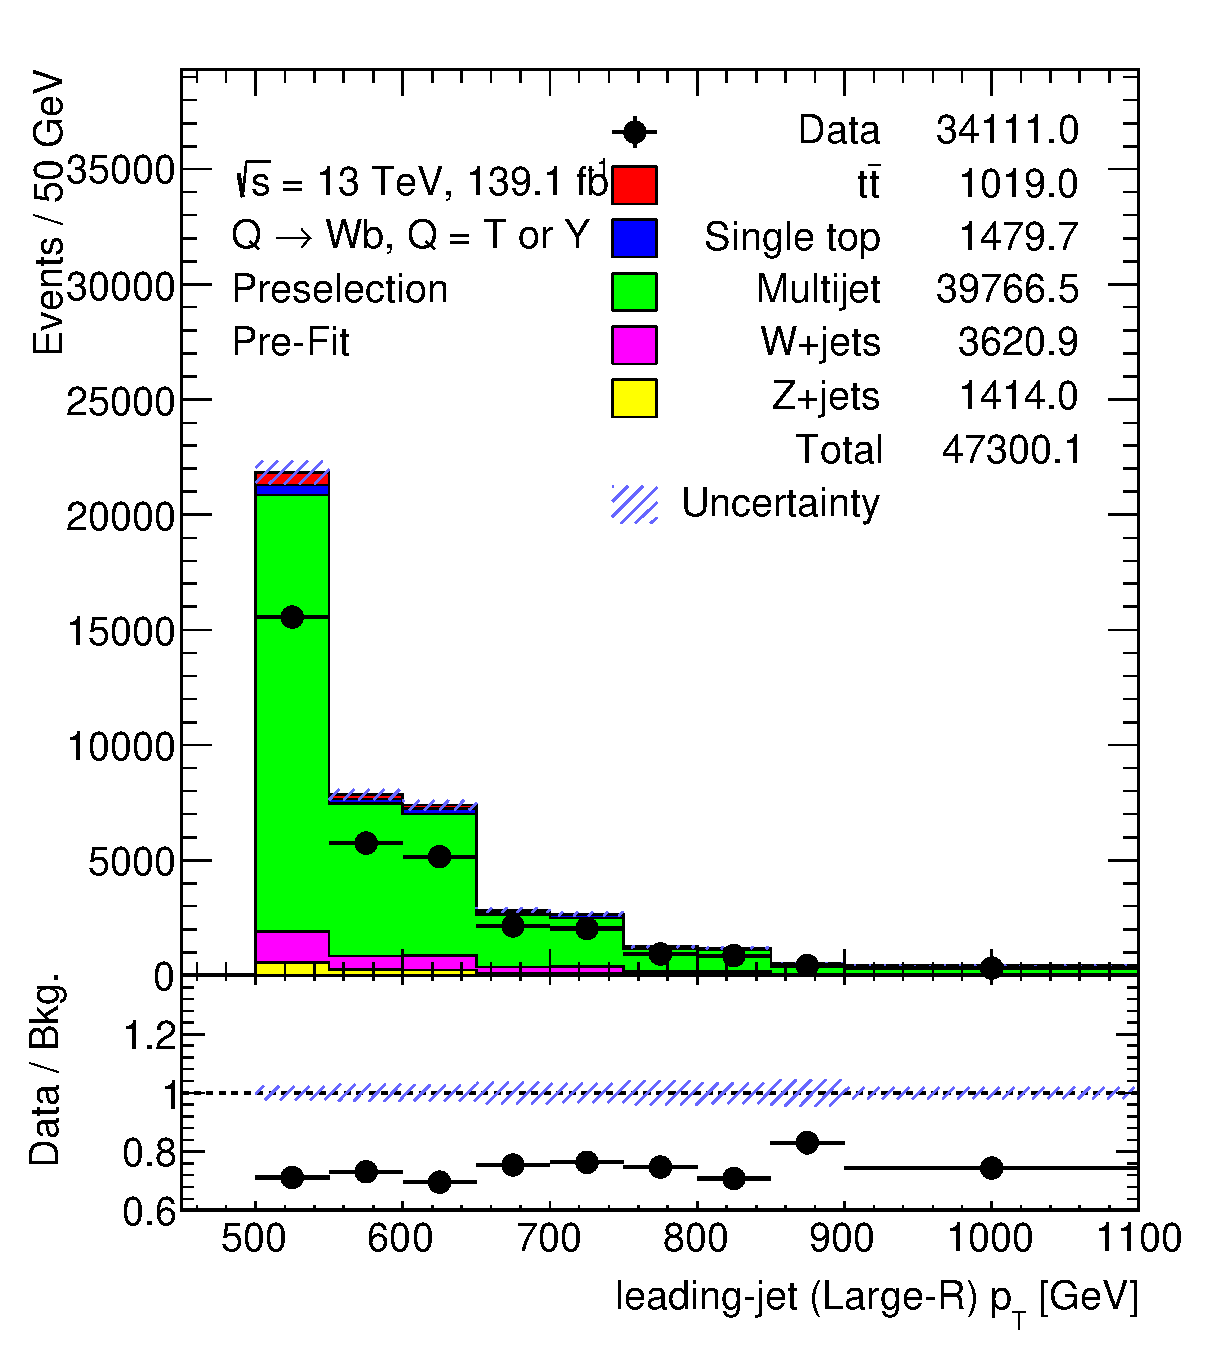
\includegraphics[width=\linewidth,height=\textheight,keepaspectratio]{Presel_ljet.eps}
		\caption{}
		\label{fig:analysisstrategy:eventselection:preselection:ljet}
	\end{subfigure}
	\begin{subfigure}{0.45\textwidth}
		\centering
		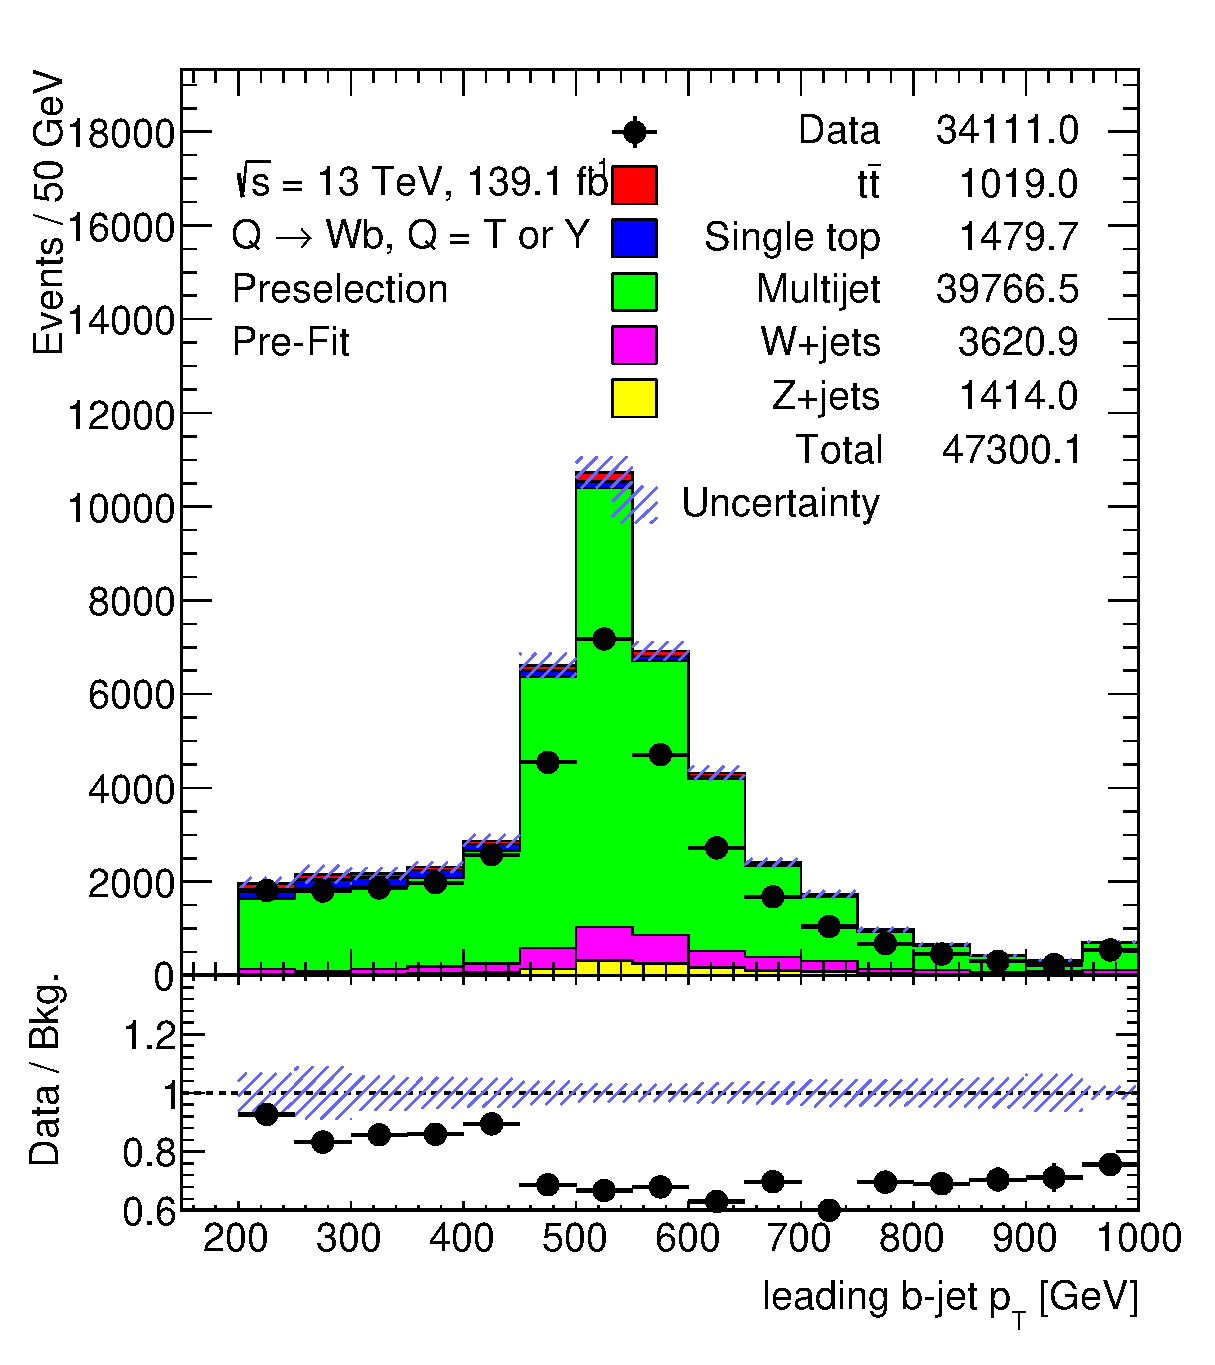
\includegraphics[width=\linewidth,height=\textheight,keepaspectratio]{Presel_bjet.eps}
		\caption{}
		\label{fig:analysisstrategy:eventselection:preselection:bjet}
	\end{subfigure}
	\begin{subfigure}{.45\textwidth}
		\centering
		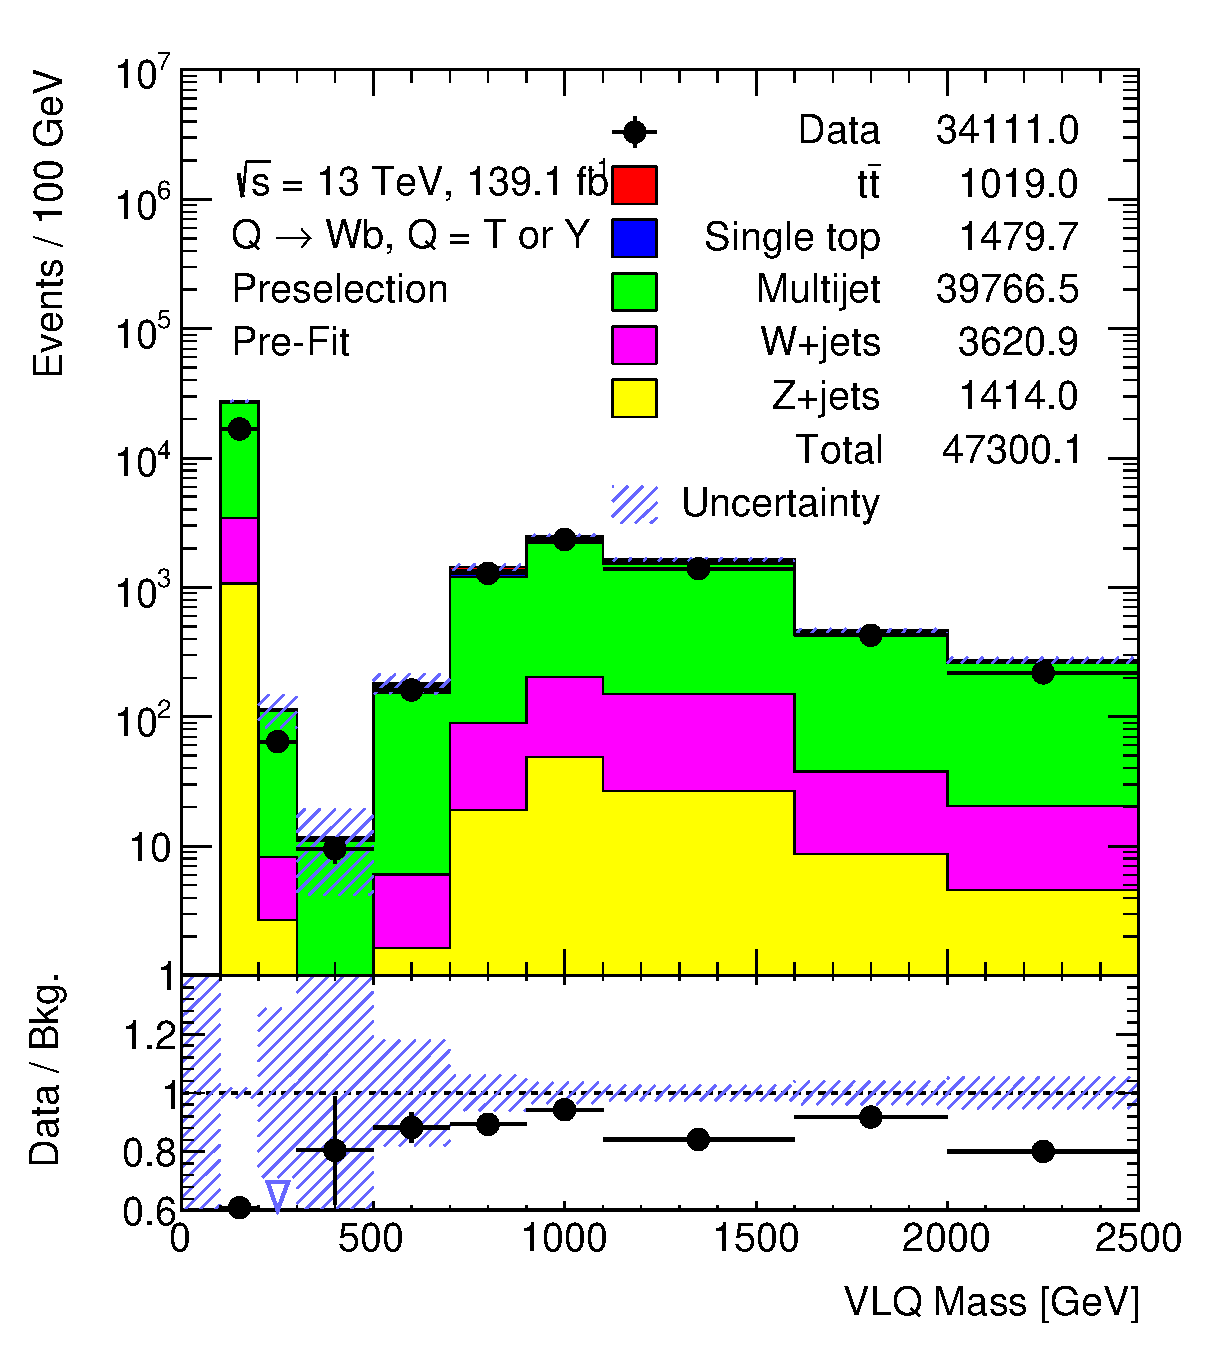
\includegraphics[width=\linewidth,height=\textheight,keepaspectratio]{Presel_VLQM.eps}
		\caption{}
		\label{fig:analysisstrategy:eventselection:preselection:vlqm}
	\end{subfigure}
	\begin{subfigure}{.45\textwidth}
		\centering
		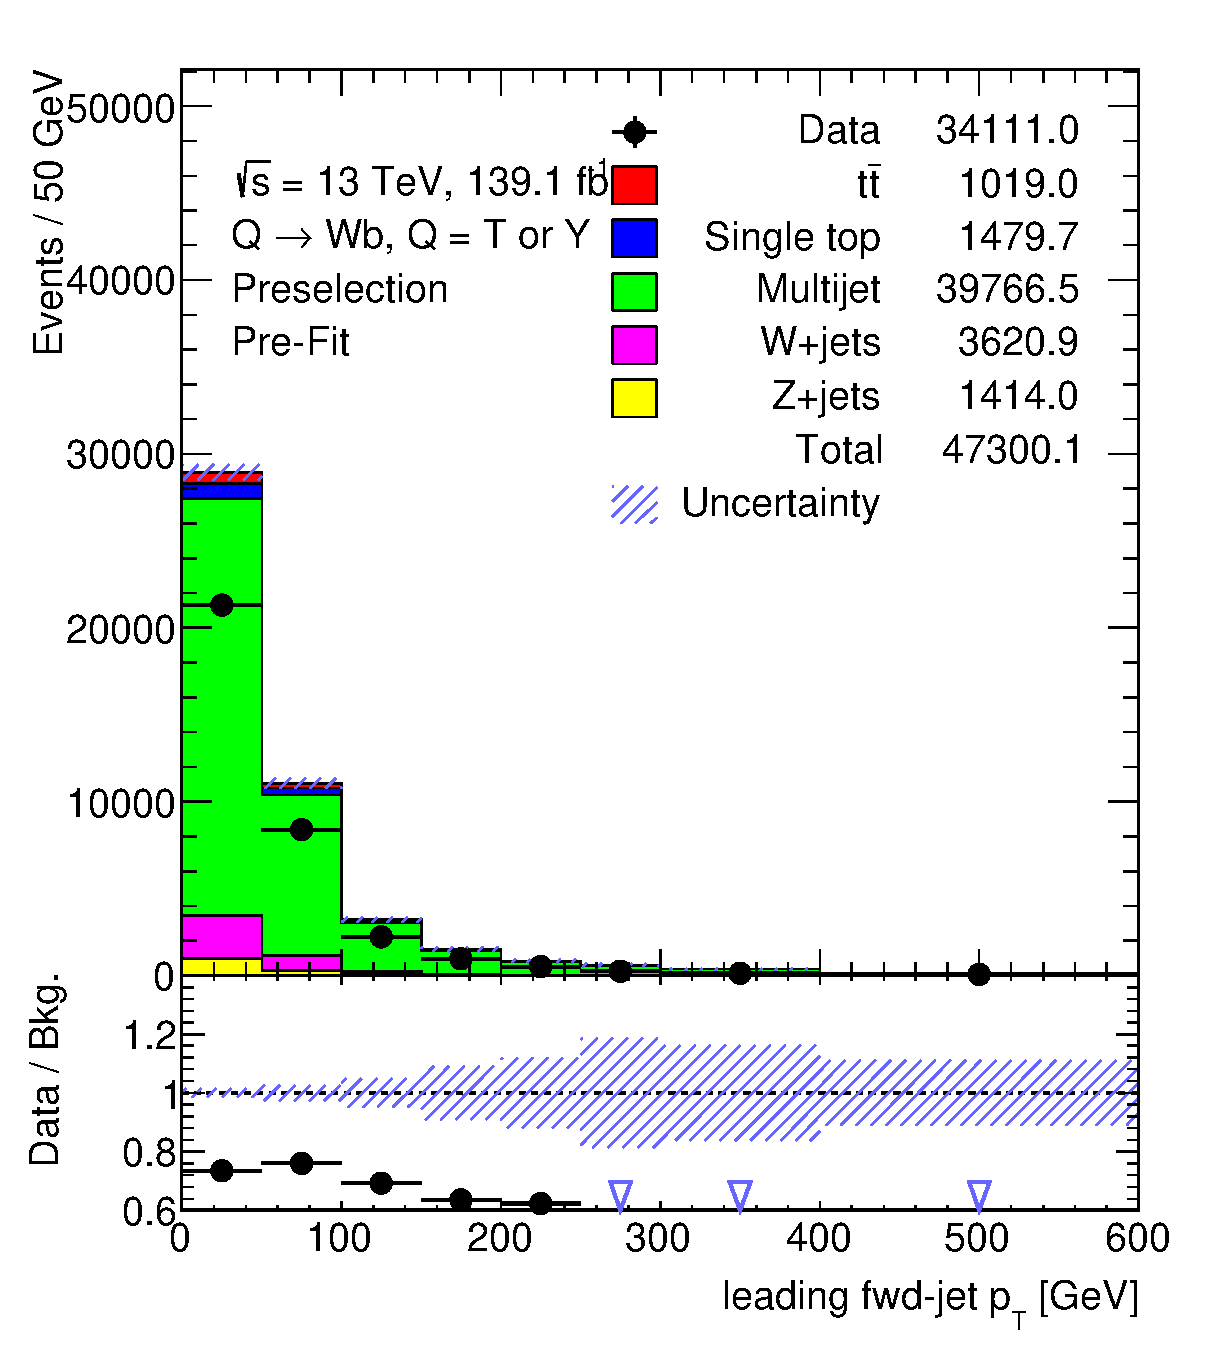
\includegraphics[width=\linewidth,height=\textheight,keepaspectratio]{Presel_fwdjet.eps}
		\caption{}
		\label{fig:analysisstrategy:eventselection:preselection:forwardjet}
	\end{subfigure}
	\caption{A data/MC comparison plots for different kinematic and reconstructed variables at the preselection level. All the backgrounds are produced from the MC simulation. It shows the distributions of (a) \pt of the $W$-tagged jet, (b) \pt of the leading $b$-tagged jet, (c) VLQ mass and (d) \pt of the leading forward jet.}
	\label{fig:analysisstrategy:eventselection:preselection}
\end{figure}

%------------------------------------------------------------------------------
\section{Need for data-driven background estimation}%
\label{sec:analysisstrategy:datadriven}
%------------------------------------------------------------------------------
The hadronic analysis is not always a clean channel because multijet is the dominant background. Multijet background comes predominantly from the QCD processes, in which a jet is identified as $W$-jet or $b$-jet. It is very difficult to model the multijet processes using the MC simulation because of the QCD effects, so it is usually mismodelled. Therefore, a better approach to estimate the multijet is needed in the hadronic analysis.

Moreover, a clear mismmodelling can be observed in the multijet MC at the preselection, as shown in Fig.\ \ref{fig:analysisstrategy:eventselection:preselection}. So, a better estimate of the multijet background is needed. In order to fix this, one can still think of scaling the multijet MC, but the ratio plots in these distributions show that just scaling the multijet MC to the data would not work. So, a dynamic approach has to be taken to predict the multijet background. This leads to perform a data-driven method for the estimation of the multijet background, which is discussed in detail in the next chapter.

